The problem of finite MDPs include evaluative feedback as seen with bandits,
but it also includes the associative aspect of linking states to actions.
We estimate $q_*(s, a)$ and $v_*(s)$, as the expected reward from taking
action $a$ in state $s$ and the maximum possible value from state $s$ respectively.

\section{The Agent-Environment Interface}
\begin{figure}[h]
    \centering
    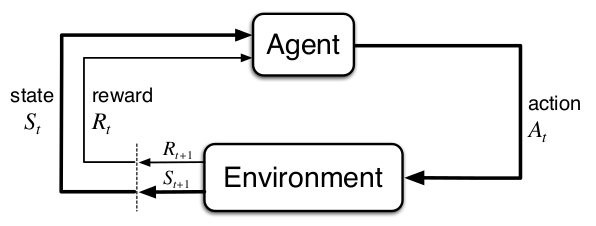
\includegraphics[width=\textwidth]{agent_env_diagram}
    \caption{The agent-environment interaction in MPDs.}
    \label{fig:3.1}
\end{figure}
At each time step $t$ the agent receives a state $s$ and then based on its
policy takes action $a$ on the environment.
Based on this action the agent receives a numerical reward from the env.
With finite MDPs the sets of $\mathcal{S}$, $\mathcal{A}$ and $\mathcal{R}$ are finite.
\begin{myequation}{3.2}
    p(s', r \mid s, a) \doteq Pr \{ S_t=s', R_t=r \mid S_{t-1}=s, A_{t-1}=a\}
\end{myequation}
\begin{myequation}{3.3}
    \sum_{s'}\sum_{r}p(s', r \mid s, a) = 1,
    \forall s \in \mathcal{S}, a \in \mathcal{A}(s)
\end{myequation}
The state must have the \textit{Markov Property} which entails that it holds
all knowledge about the past agent-env interaction that makes a difference
moving forward.
\begin{myequation}{3.4}
    p(s' \mid s,a) \doteq Pr\{S_t = s' \mid S_{t-1} = s, A_{t-1} = a\} =
    \sum_{r} p(s', r \mid s, a)
\end{myequation}
\begin{myequation}{3.5}
    r(s, a) \doteq \mathbb{E}\left[R_t \mid S_{t-1}=s, A_{t-1}=a\right] =
    \sum_{r} r \sum_{s'} p(s', r \mid s, a)
\end{myequation}
\begin{myequation}{3.6}
    r(s, a, s') \doteq
    \mathbb{E}\left[R_t \mid S_{t-1}=s, A_{t-1}=a, S{t}=s'\right] =
    \sum_{r}r \cdot p(s',r \mid s, a)
\end{myequation}

\section{Goals and Rewards}
    The reward signal is your way of communicating to the robot what you want
    it to achieve, not how you want it achieved.

\section{Returns and Episodes}
We define return after step $t$ as
\begin{myequation}{3.7}
    G_t\doteq R_{t+1}+R{t+2}+...+R_T=\sum_{k=0}^{T}R_{t+k+1}
\end{myequation}
\begin{itemize*}
    \item $T$: the terminal state.
    \item $R_t$: reward at time $t$.
\end{itemize*}
We define discounted return for non episodic tasks as:
\begin{myequation}{3.8}
    G_t\doteq \sum_{k=0}^{\infty}\gamma^kR_{t+k+1}
\end{myequation}
\begin{myequation}{3.9}
    G_t\doteq R_{t+1} + \gamma G_{t+1}
\end{myequation}
\begin{itemize*}
    \item $\gamma \in [0, 1]$: the discount rate.
\end{itemize*}
If the reward is a constant +1:
\begin{myequation}{3.10}
    G_t\doteq \sum_{k=0}^{\infty}\gamma^k=\frac{1}{1-\gamma}
\end{myequation}

\section{Unified Notation for Episodic and Continuing Tasks}

\section{Policies and Value Functions}
\textbf{Value functions} show how good a state is, or how good of a move would be to
take an action $a$ at state $s$.
\textbf{Policy} is a mapping from state $s$ to probabilities of taking actions in $A$.

\begin{exercise}{3.11}
    If the current state is $S_t$, and actions are selected
    according to stochastic policy $\pi$, then what is the expectation of $R_{t+1}$
    in terms of $\pi$ and the four-argument function $p$ \hyperref[eq:3.2]{(3.2)}?
    \begin{equation*}
        R_{t+1} = \sum_a \pi(a\mid s)\sum_{s',r}p(s',r\mid a,s)
    \end{equation*}
\end{exercise}

For \hyperref[def:mdp]{MDP}s we define $v_{\pi}$ as the
\textit{state-value function for policy $\pi$}:

\begin{myequation}{3.12}
    \begin{aligned}
        v_{\pi}(s) &\doteq \mathbb{E}_{\pi} \left[G_t \mid S_t = s \right] \\
        &=\mathbb{E}_{\pi}\left[\sum_{k=0}^{\infty}\gamma^k R_{t+k+1} \mid S_t = s\right]
        , \forall s \in \mathcal{S}
    \end{aligned}
\end{myequation}

And $q_{\pi}(s, a)$ as the \textit{action-value function for policy $\pi$}:

\begin{myequation}{3.13}
    \begin{aligned}
        q_{\pi}(s, a) &\doteq \mathbb{E}_{\pi}\left[G_t \mid S_t=s, A_t=a\right] \\
        &=\mathbb{E}_{\pi}\left[\sum_{k=0}^{\infty}\gamma^k R_{t+k+1} \mid S_t=s, A_t=a\right]
    \end{aligned}
\end{myequation}

\begin{exercise}{3.12}
    Give an equation for $v_{\pi}$ in terms of $q_{\pi}$ and $\pi$.
    \begin{equation*}
        v_{\pi} = \sum_a \pi(a\mid s)\cdot q_{\pi}(a, s)
    \end{equation*}
\end{exercise}

\begin{exercise}{3.13}
    Give an equation for $q_{\pi}$ in terms of $v_{\pi}$
    and the four-argument $p$.
    \begin{equation*}
        q_{\pi} = \sum_{s'} v_{\pi}(s') \sum_r p(s',r\mid a,s)
    \end{equation*}
\end{exercise}

\textit{Monte Carlo methods} are RL methods that involve averaging over many random
samples for the actual returns.

\begin{myequation}{3.14}
    \begin{aligned}
        v_{\pi}(s) &\doteq \mathbb{E}_{\pi}\left[G_t \mid S_t=s\right]\\
        &=\mathbb{E}_{\pi}\left[R_{t+1}+\gamma G_{t+1} \mid S_t=s \right] \\
        &=\sum_a \pi(a \mid s) \sum_{s'}\sum_r p(s', r \mid s, a)
        \left[r+\gamma \mathbb{E}_{\pi}\left[G_{t+1}\mid S_{t+1}=s'\right]\right] \\
        &=\sum_a \pi(a \mid s) \sum_{s', r}p(s', r \mid s, a)\left[r+\gamma v_{\pi}(s')\right],
        \forall s \in \mathcal{S}
    \end{aligned}
\end{myequation}

This last equation is the so-called \textit{Bellman equation for $v_{\pi}$} and is essentially
weighing the values in the brackets on the right given the probability \newline
\mbox{$\pi(a\mid s)p(s',r\mid s, a)$}, and iterating through all possibilities.

\begin{figure}[h]
    \centering
    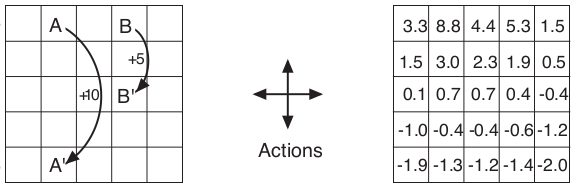
\includegraphics[scale=0.5]{grid_world_ex}
    \caption{Gridworld example: exceptional reward dynamics (left) and state-value function
    for the equiprobable random policy (right).
    Suppose the agent selects all four actions (left, right, up, down) with equal
    probability in all states.
    $\gamma=0.9$.}
    \label{fig:3.2}
\end{figure}

\begin{exercise}{3.17}
    \begin{wrapfigure}{r}{0.3\linewidth}
        \centering
        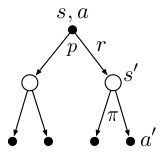
\includegraphics[scale=0.6]{action_value_backup_diagram.png}
    \end{wrapfigure}
    What is the Bellman equation for action values, that is, for $q_{\pi}$?
    It must give the action value $q_{\pi}(s, a)$ in terms of the action
    values, $q_{\pi}(s',a')$, of possible successors to the state-action pair $(s, a)$.
    Hint: The diagram corresponds to this equation.
    Show the sequence of equations analogous to \hyperref[eq:3.14]{(3.14)}, but for action
    values.
    \[
        \begin{aligned}
            q_{\pi}(s,a)
            &=\mathbb{E}_{\pi}\left[\sum_{k=0}^{\infty}\gamma^k R_{t+k+1} \mid S_t=s, A_t=a\right]\\
            &=\sum_{s',r}p(s',r\mid a, s)\cdot r
            + \sum_{s'}p(s'\mid s,a)\cdot\gamma\sum_{a'}\pi (a'|s')\cdot q_{\pi}(s',a')
        \end{aligned}
    \]
\end{exercise}

\begin{exercise}{3.18}
    \begin{center}
        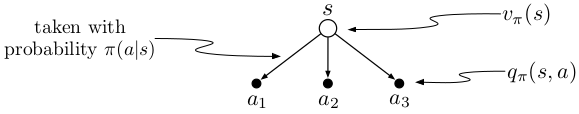
\includegraphics[scale=0.5]{exercise_3_18_diagram}
    \end{center}
    Give the equation corresponding to the root node, $v_{\pi}(s)$, in terms of the
    value at the expected leaf node, $q_{\pi}(s, a)$, given $S_t=s$.
    This equation should include an expectation conditioned on following the policy $\pi$.
    Then give a second equation in which the expected value is written out explicitly
    in terms of $\pi(a|s)$ such that no expected value notation appears in the equation.
    \[
        \begin{aligned}
            v_{\pi}(s)&=\mathbb{E}_{\pi}\left[q_{\pi}(s,a)\right]\\
            &=\sum_{a}\pi(a\mid s)\cdot q_{\pi}(s,a)
        \end{aligned}
    \]
\end{exercise}

\begin{exercise}{3.19}
    \begin{center}
        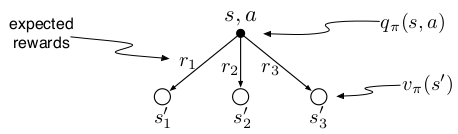
\includegraphics[scale=0.5]{exercise_3_19_diagram}
    \end{center}
    Give the equation corresponding to this intuition and diagram for the action value,
    $q_{\pi}(s,a)$, in terms of the expected new reward, $r_{t+1}$, and the expected
    next state value, $v_{\pi}(s_{t+1})$, given $s_t$ and $a_t$.
    This equation should include an expectation but not one condition on following the policy.
    Then give a second equation, writing out the expected value explicitly in terms of
    $p(s',r\mid s,a)$ defined by \hyperref[eq:3.2]{(3.2)}, such that no expected value notation
    appears in the equation.
    \[
        \begin{aligned}
            q_{\pi}(s,a)&=\mathbb{E}_{s,a}\left[r_{t+1}+\gamma v_{\pi}(s')\right]\\
            &=\sum_{s',r}p(s',r\mid s,a)\cdot r + \gamma\sum_{s'}p(s'\mid s,a)\cdot v_{\pi}(s')
        \end{aligned}
    \]
\end{exercise}

\section{Optimal Policies and Optimal Value Functions}
A policy $\pi'$ is better than policy $\pi$ if $\forall s \in \mathcal{S}, v_{\pi'}\geq v_{\pi}$.
In other words
\[
    \pi'\geq \pi \Longleftrightarrow (\forall s\in\mathcal{S})(v_{\pi'}\geq v_{\pi})
\]

\textit{Optimal policy}:
\begin{myequation}{3.60*}
    \pi_*\doteq \max_{v_{\pi}(s)}\pi,\forall s\in\mathcal{S}
\end{myequation}
\textit{Optimal state-value function}:
\begin{myequation}{3.15}
    v_*(s)\doteq \max_{\pi}v_{\pi}(s),\forall s\in\mathcal{S}
\end{myequation}
\textit{Optimal action-value function}:
\begin{myequation}{3.16}
    q_*(s,a)\doteq \max_{\pi}q_{\pi}(a,s),\forall s\in\mathcal{S},\forall a\in\mathcal{A}
\end{myequation}
\begin{myequation}{3.17}
    q_*(s,a)=\mathbb{E}\left[R_{t+1}+\gamma v_*(S_{t+1})\in S_t=s,A_t=a\right]
\end{myequation}
\textit{Bellman optimality equation}:
\begin{myequation}{3.18}
    \begin{aligned}
        v_*(s)&=\max_{a\in\mathcal{A}(s)}q_{\pi_*}(s,a)\\
        &=\max_a\mathbb{E}_{\pi_*}\left[G_t\mid S_t=s,A_t=a\right]\\
        &=\max_a\mathbb{E}\left[R_{t+1}+\gamma v_*(S_{t+1})\mid S_t=s,A_t=a\right]\\
        &=\max_a\sum_{s',r}p(s',r\mid s,a)[r+\gamma v_*(s')]
    \end{aligned}
\end{myequation}
\begin{myequation}{3.20}
    \begin{aligned}
        q_*(s,a)&=\mathbb{E}\left[
            R_{t+1}+\gamma\max_{a'}q_*(S_{t+1},a')\mid S_t=s,A_t=a
        \right]\\
        &=\sum_{s',r}p(s',r\mid s,a)\left[r+\gamma\max_{a'}q_*(s',a')\right]
    \end{aligned}
\end{myequation}

Solving the \textit{Bellman optimality equations} relies on having having the following three
properties that are rarely found in real-world scenarios:
\begin{itemize}
    \item accurate knowledge of the dynamics of the environment.
    \item computational resources to complete the computation of the solution.
    \item the Markov property.
\end{itemize}

\begin{exercise}{3.25}
    Give an equation for $v_*$ in terms of $q_*$.
    \[
        v_*(s) = \max_a q_*(s,a)
    \]
\end{exercise}
\begin{exercise}{3.26}
    Give an equation for $q_*$ in terms of $v_*$ and the four-argument
    $p$ \hyperref[eq:3.2]{(3.2)}.
    \[
        q_*(s, a) = \sum_{s',r}p(s',r\mid s,a)\cdot(r + \gamma v_*(s'))
    \]
\end{exercise}
\begin{exercise}{3.29 !?}
    Rewrite the four Bellman equations for the four value functions
    ($v_{\pi}, v_*, q_{\pi}, q_*$) in terms of the three-argument
    function $p$ \hyperref[eq:3.4]{(3.4)} and the two-argument
    function $r$ \hyperref[eq:3.5]{(3.5)}.
    \[
        \begin{aligned}
            v_{\pi}(s)&=\sum_a\pi(a\mid s)
            \sum_{s', r}p(s',r\mid s,a)\left[r+\gamma v_{\pi}(s')\right] \\
            &=\sum_a\pi(a\mid s)\cdot r(s,a)\cdot\gamma
            \sum_{s'}p(s'\mid s,a)]\cdot v_{\pi}(s') \\
        \end{aligned}
    \]
\end{exercise}

\section{Optimality and Approximation}
Tabular methods can store the optimal policy in a table but a lot of RL problems have
a huge number of states that cannot be represented through a table due to memory restrictions.
Therefore, we resolve to approximation methods.


\section{Summary}
\label{sec:fmdps-summary}
Let us summarize the elements of the reinforcement learning problem that we have
presented in this chapter. Reinforcement learning is about learning from interaction
how to behave in order to achieve a goal. The reinforcement learning agent and its
environment interact over a sequence of discrete time steps. The specification of their
interface defines a particular task: the actions are the choices made by the agent; the
states are the basis for making the choices; and the rewards are the basis for evaluating
the choices. Everything inside the agent is completely known and controllable by the
agent; everything outside is incompletely controllable but may or may not be completely
known. A policy is a stochastic rule by which the agent selects actions as a function of
states. The agent’s objective is to maximize the amount of reward it receives over time.
When the reinforcement learning setup described above is formulated with well defined
transition probabilities it constitutes a Markov decision process (MDP). A finite MDP is
an MDP with finite state, action, and (as we formulate it here) reward sets. Much of the
current theory of reinforcement learning is restricted to finite MDPs, but the methods
and ideas apply more generally.
The return is the function of future rewards that the agent seeks to maximize (in
expected value). It has several different definitions depending upon the nature of the
task and whether one wishes to discount delayed reward. The undiscounted formulation
is appropriate for episodic tasks, in which the agent–environment interaction breaks
naturally into episodes; the discounted formulation is appropriate for continuing tasks, in
which the interaction does not naturally break into episodes but continues without limit.
We try to define the returns for the two kinds of tasks such that one set of equations can
apply to both the episodic and continuing cases.
A policy’s value functions assign to each state, or state–action pair, the expected return
from that state, or state–action pair, given that the agent uses the policy. The optimal
value functions assign to each state, or state–action pair, the largest expected return
achievable by any policy. A policy whose value functions are optimal is an optimal policy.
Whereas the optimal value functions for states and state–action pairs are unique for a
given MDP, there can be many optimal policies. Any policy that is greedy with respect to
the optimal value functions must be an optimal policy. The Bellman optimality equations
are special consistency conditions that the optimal value functions must satisfy and that
can, in principle, be solved for the optimal value functions, from which an optimal policy
can be determined with relative ease.
A reinforcement learning problem can be posed in a variety of different ways depending
on assumptions about the level of knowledge initially available to the agent. In problems
of complete knowledge, the agent has a complete and accurate model of the environment’s
dynamics. If the environment is an MDP, then such a model consists of the complete four-
argument dynamics function $p$ (\ref{eq:3.2}).
In problems of incomplete knowledge, a complete
and perfect model of the environment is not available.
Even if the agent has a complete and accurate environment model, the agent is
typically unable to perform enough computation per time step to fully use it. The
memory available is also an important constraint. Memory may be required to build
up accurate approximations of value functions, policies, and models. In most cases of
practical interest there are far more states than could possibly be entries in a table, and
approximations must be made.
A well-defined notion of optimality organizes the approach to learning we describe in
this book and provides a way to understand the theoretical properties of various learning
algorithms, but it is an ideal that reinforcement learning agents can only approximate
to varying degrees. In reinforcement learning we are very much concerned with cases in
which optimal solutions cannot be found but must be approximated in some way.
